\section{Fase 2: Planeación de actividades}
En esta fase el \textit{Data Analysis Team} basado en las preguntas realizadas en el BCQM analiza todas las tareas que hay que llevar a cabo, las estiman en tiempo y las distribuyen entre las personas que las van a realizar durante el \textit{Release}. Dado que el BCQM nos permite conocer de antemano el tipo de cáncer de mama y la técnica para el diagnostico de esta enfermedad, el científico de datos con ayuda del medico puede definir el origen de datos, lo cual va a permitir conocer el tipo, cantidad y peso de la información. Dado lo anterior, es recomendable que el equipo tenga al menos un ingeniero datos, ya que el es el encargado de tomar los datos y convertirlos en información significativa para que el científico pueda realizar el respectivo análisis.  

\begin{figure}[!htb]
	\centering
	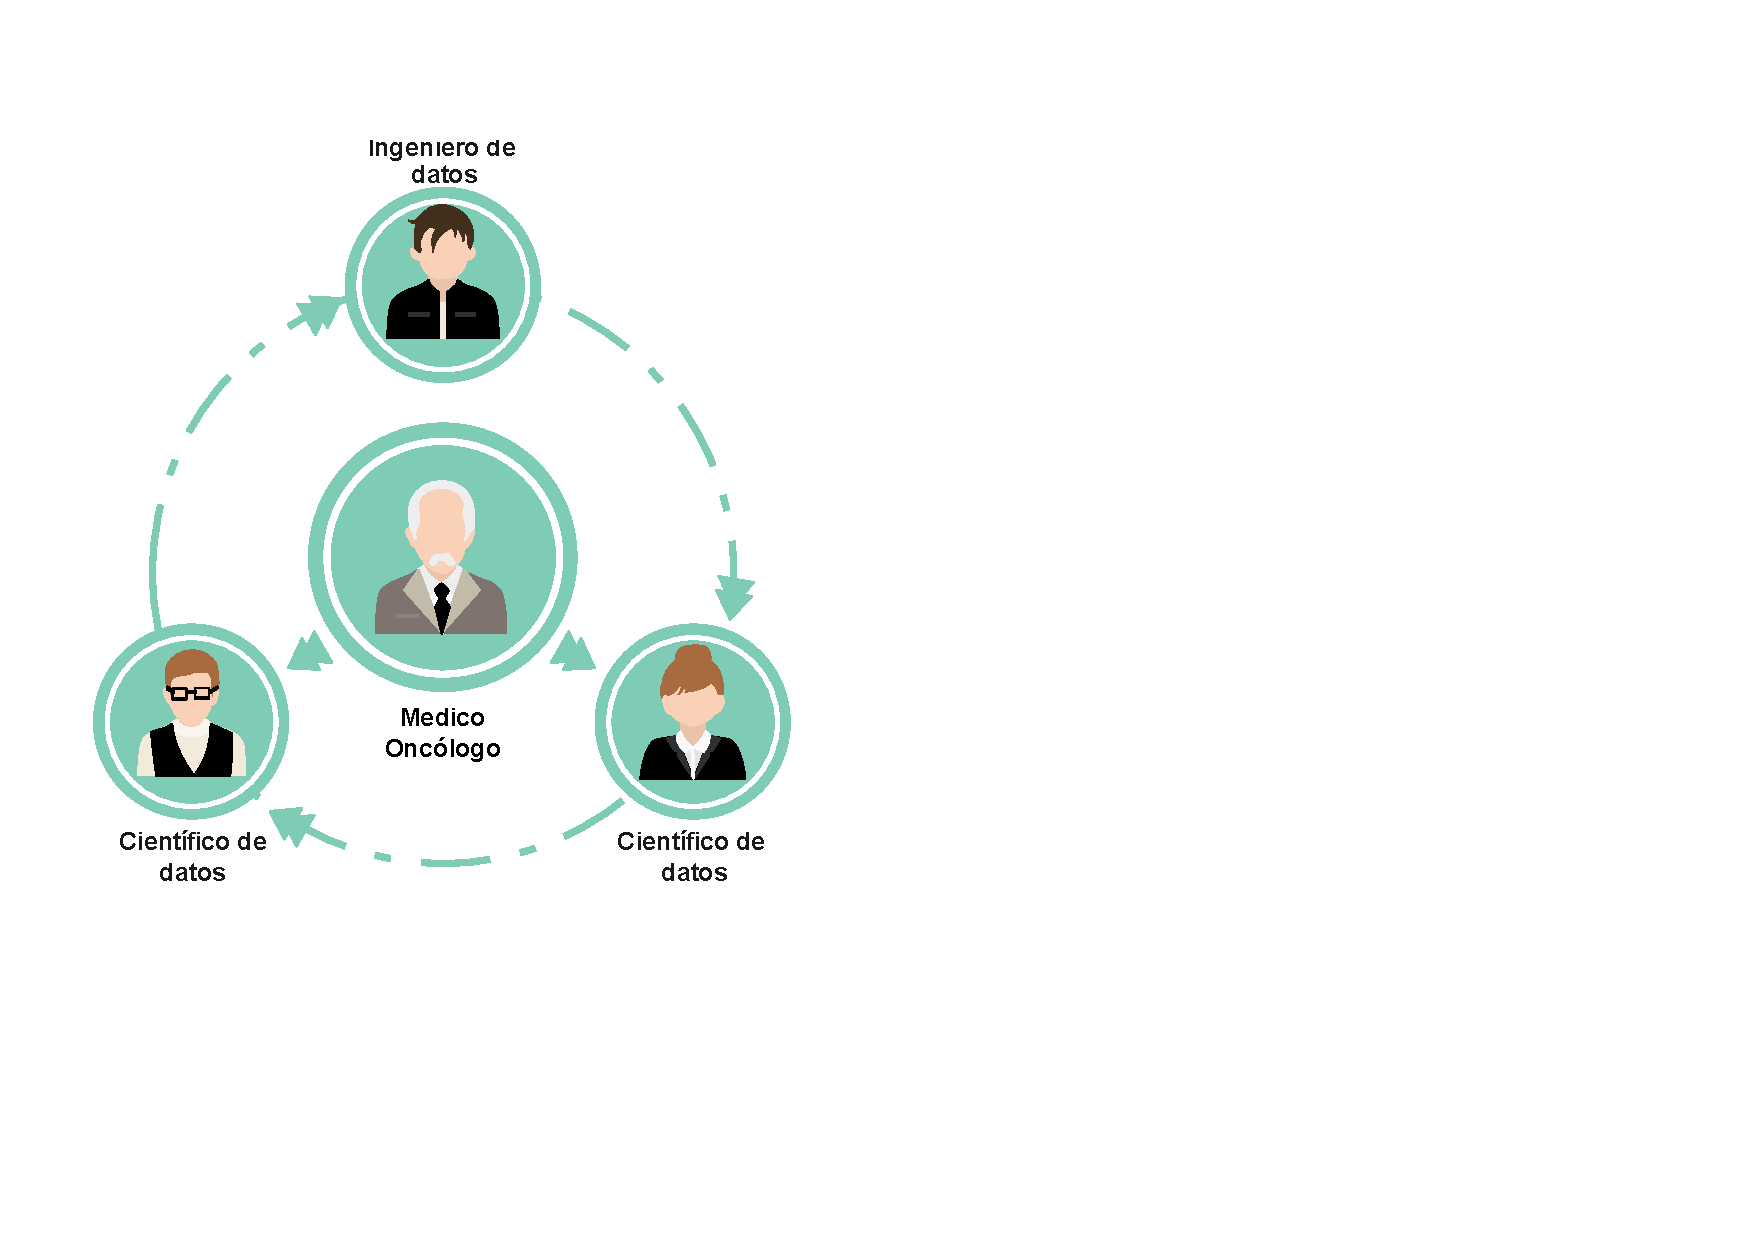
\includegraphics[width=0.36
	\linewidth]{IMAGENES/Data_Analysis_Team}
	\caption{Conformación del Data Analysis Team. }
	\label{Data_Analysis_Team}
\end{figure}

\begin{figure}[!htb]
	\centering
	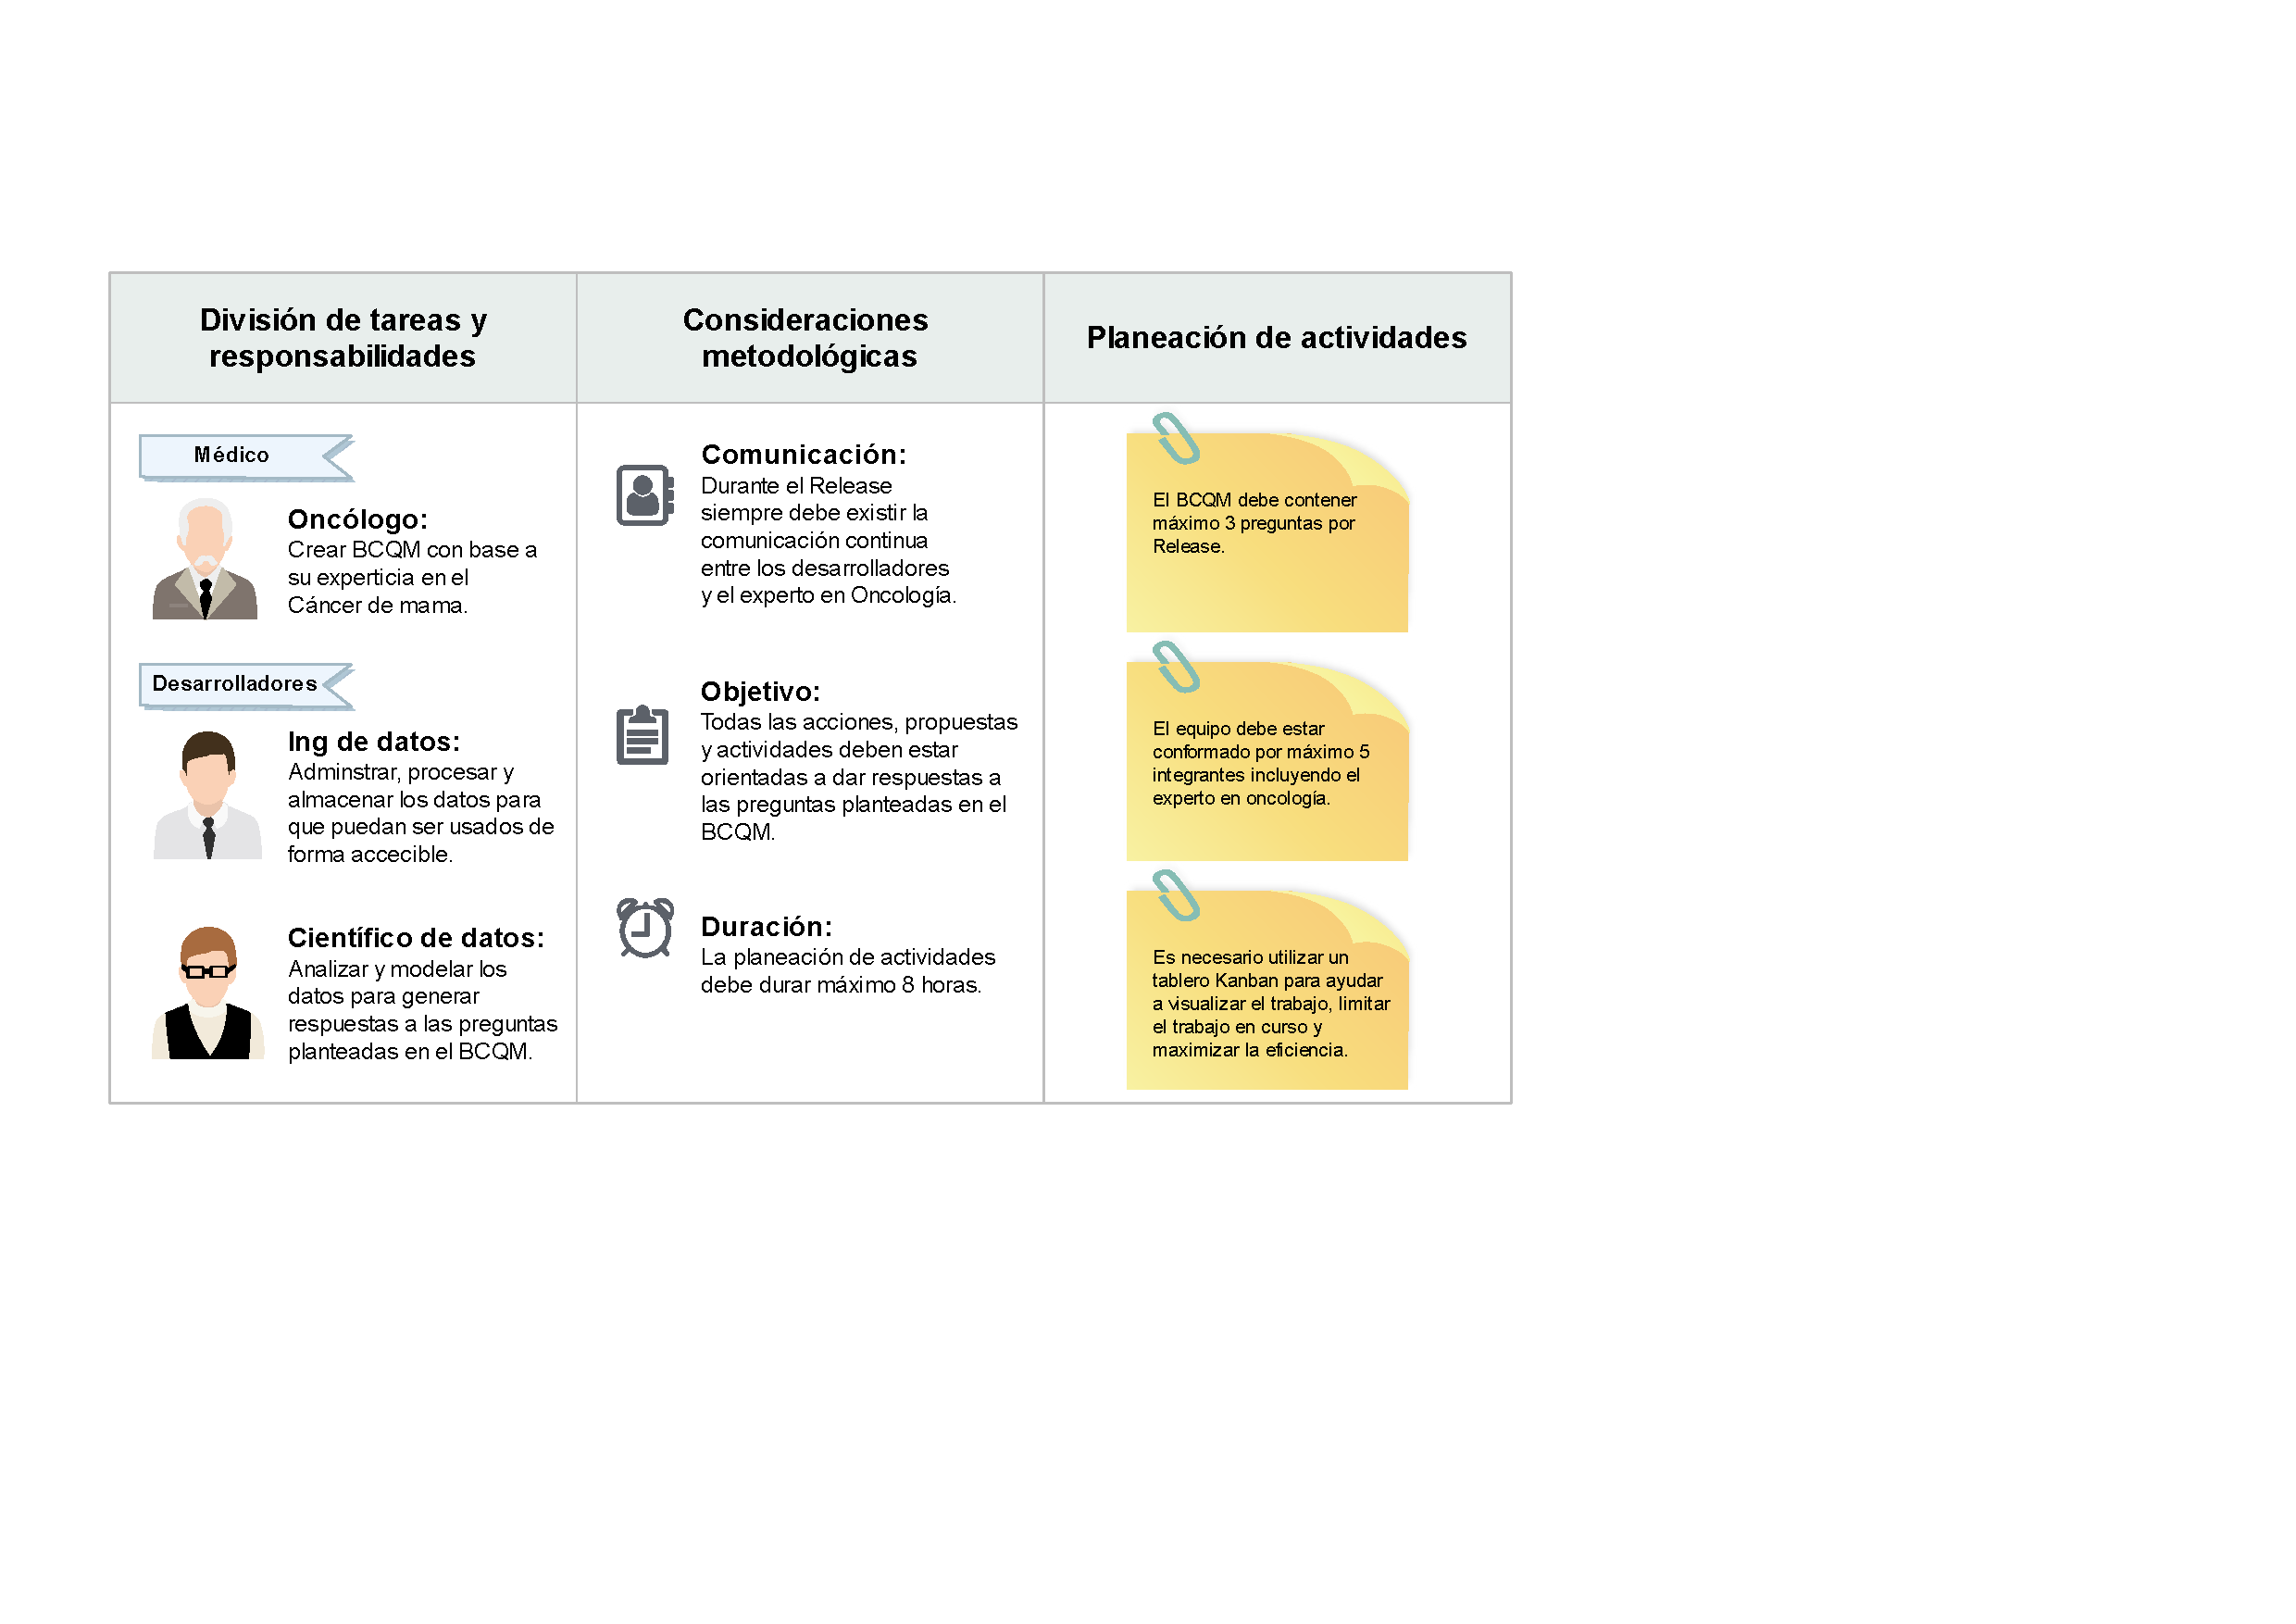
\includegraphics[width=0.68
	\linewidth]{IMAGENES/Activity_Planning}
	\caption{Planeación de actividades realizada por el Data Analysis Team. }
	\label{Activity_Planning}
\end{figure}

 Una vez generadas las preguntas en el BCQM es posible que varias actividades este relacionadas a varias preguntas, por lo tanto se recomienda al \textit{Data Analysis Team} agrupar en una sola actividad las tareas a realizar para generar una mayor agilidad en la elaboración de interpretaciones y respuestas. Así mismo todas las acciones, propuestas y actividades deben estar orientadas en generar respuestas a las preguntas planteadas, siendo el principal objetivo que el experto en oncologia tome una decisión de valor. Dado lo anterior, durante el Release siempre debe existir una comunicación continua y efectiva entre el equipo técnico y el experto en oncologia. Finalmente, la planeación de actividades debe durar máximo 8 horas y su creación debe estar de acuerdo a las habilidades técnicas de cada participante del equipo.
 
Para un mayor entendimiento, basados en las 3 preguntas planteadas en el BCQM, se genero la siguiente planeación de actividades para generar respuestas basados en los datos de índole genómico responsables del desarrollo del cáncer de mama:
\begin{figure}[!htb]
	\centering
	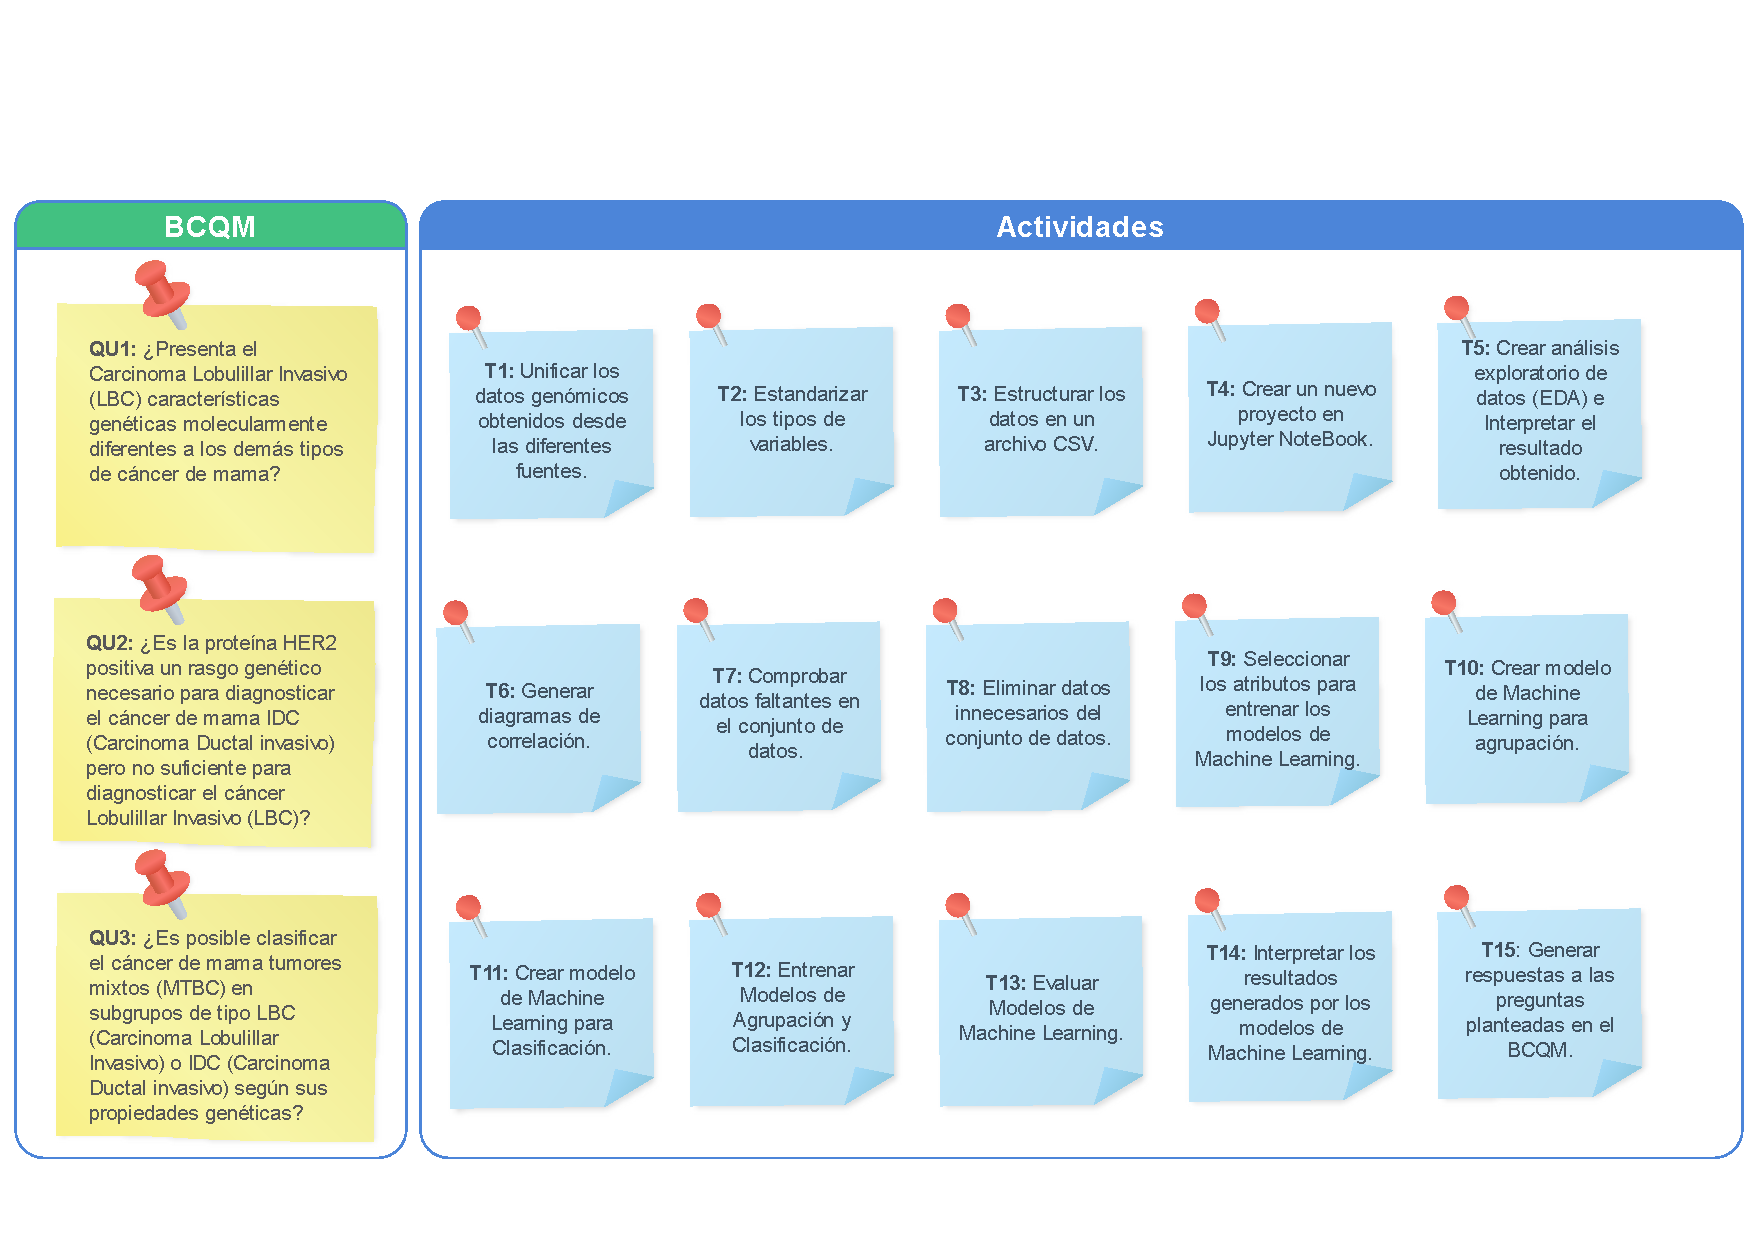
\includegraphics[width=
	\linewidth]{IMAGENES/Planning_TCGA}
	\caption{Planeación de actividades realizada por el Data Analysis Team. }
	\label{Activity_Planning_TCGA}
\end{figure}
